% GNUPLOT: LaTeX picture with Postscript
\begingroup
  \makeatletter
  \providecommand\color[2][]{%
    \GenericError{(gnuplot) \space\space\space\@spaces}{%
      Package color not loaded in conjunction with
      terminal option `colourtext'%
    }{See the gnuplot documentation for explanation.%
    }{Either use 'blacktext' in gnuplot or load the package
      color.sty in LaTeX.}%
    \renewcommand\color[2][]{}%
  }%
  \providecommand\includegraphics[2][]{%
    \GenericError{(gnuplot) \space\space\space\@spaces}{%
      Package graphicx or graphics not loaded%
    }{See the gnuplot documentation for explanation.%
    }{The gnuplot epslatex terminal needs graphicx.sty or graphics.sty.}%
    \renewcommand\includegraphics[2][]{}%
  }%
  \providecommand\rotatebox[2]{#2}%
  \@ifundefined{ifGPcolor}{%
    \newif\ifGPcolor
    \GPcolortrue
  }{}%
  \@ifundefined{ifGPblacktext}{%
    \newif\ifGPblacktext
    \GPblacktexttrue
  }{}%
  % define a \g@addto@macro without @ in the name:
  \let\gplgaddtomacro\g@addto@macro
  % define empty templates for all commands taking text:
  \gdef\gplbacktext{}%
  \gdef\gplfronttext{}%
  \makeatother
  \ifGPblacktext
    % no textcolor at all
    \def\colorrgb#1{}%
    \def\colorgray#1{}%
  \else
    % gray or color?
    \ifGPcolor
      \def\colorrgb#1{\color[rgb]{#1}}%
      \def\colorgray#1{\color[gray]{#1}}%
      \expandafter\def\csname LTw\endcsname{\color{white}}%
      \expandafter\def\csname LTb\endcsname{\color{black}}%
      \expandafter\def\csname LTa\endcsname{\color{black}}%
      \expandafter\def\csname LT0\endcsname{\color[rgb]{1,0,0}}%
      \expandafter\def\csname LT1\endcsname{\color[rgb]{0,1,0}}%
      \expandafter\def\csname LT2\endcsname{\color[rgb]{0,0,1}}%
      \expandafter\def\csname LT3\endcsname{\color[rgb]{1,0,1}}%
      \expandafter\def\csname LT4\endcsname{\color[rgb]{0,1,1}}%
      \expandafter\def\csname LT5\endcsname{\color[rgb]{1,1,0}}%
      \expandafter\def\csname LT6\endcsname{\color[rgb]{0,0,0}}%
      \expandafter\def\csname LT7\endcsname{\color[rgb]{1,0.3,0}}%
      \expandafter\def\csname LT8\endcsname{\color[rgb]{0.5,0.5,0.5}}%
    \else
      % gray
      \def\colorrgb#1{\color{black}}%
      \def\colorgray#1{\color[gray]{#1}}%
      \expandafter\def\csname LTw\endcsname{\color{white}}%
      \expandafter\def\csname LTb\endcsname{\color{black}}%
      \expandafter\def\csname LTa\endcsname{\color{black}}%
      \expandafter\def\csname LT0\endcsname{\color{black}}%
      \expandafter\def\csname LT1\endcsname{\color{black}}%
      \expandafter\def\csname LT2\endcsname{\color{black}}%
      \expandafter\def\csname LT3\endcsname{\color{black}}%
      \expandafter\def\csname LT4\endcsname{\color{black}}%
      \expandafter\def\csname LT5\endcsname{\color{black}}%
      \expandafter\def\csname LT6\endcsname{\color{black}}%
      \expandafter\def\csname LT7\endcsname{\color{black}}%
      \expandafter\def\csname LT8\endcsname{\color{black}}%
    \fi
  \fi
    \setlength{\unitlength}{0.0500bp}%
    \ifx\gptboxheight\undefined%
      \newlength{\gptboxheight}%
      \newlength{\gptboxwidth}%
      \newsavebox{\gptboxtext}%
    \fi%
    \setlength{\fboxrule}{0.5pt}%
    \setlength{\fboxsep}{1pt}%
\begin{picture}(8640.00,11520.00)%
    \gplgaddtomacro\gplbacktext{%
      \colorrgb{0.00,0.00,0.00}%%
      \put(750,7475){\makebox(0,0)[r]{\strut{}}}%
      \colorrgb{0.00,0.00,0.00}%%
      \put(750,8165){\makebox(0,0)[r]{\strut{}0.2}}%
      \colorrgb{0.00,0.00,0.00}%%
      \put(750,8855){\makebox(0,0)[r]{\strut{}0.4}}%
      \colorrgb{0.00,0.00,0.00}%%
      \put(750,9544){\makebox(0,0)[r]{\strut{}0.6}}%
      \colorrgb{0.00,0.00,0.00}%%
      \put(750,10234){\makebox(0,0)[r]{\strut{}0.8}}%
      \colorrgb{0.00,0.00,0.00}%%
      \put(750,10924){\makebox(0,0)[r]{\strut{}1}}%
      \colorrgb{0.00,0.00,0.00}%%
      \put(1228,7271){\makebox(0,0){\strut{}}}%
      \colorrgb{0.00,0.00,0.00}%%
      \put(1961,7271){\makebox(0,0){\strut{}}}%
      \colorrgb{0.00,0.00,0.00}%%
      \put(2693,7271){\makebox(0,0){\strut{}}}%
      \colorrgb{0.00,0.00,0.00}%%
      \put(3425,7271){\makebox(0,0){\strut{}}}%
      \colorrgb{0.00,0.00,0.00}%%
      \put(4158,7271){\makebox(0,0){\strut{}}}%
      \csname LTb\endcsname%%
      \put(3425,10579){\makebox(0,0)[l]{\strut{}ZPE300}}%
    }%
    \gplgaddtomacro\gplfronttext{%
    }%
    \gplgaddtomacro\gplbacktext{%
      \colorrgb{0.00,0.00,0.00}%%
      \put(4413,7475){\makebox(0,0)[r]{\strut{}}}%
      \colorrgb{0.00,0.00,0.00}%%
      \put(4413,8165){\makebox(0,0)[r]{\strut{}}}%
      \colorrgb{0.00,0.00,0.00}%%
      \put(4413,8855){\makebox(0,0)[r]{\strut{}}}%
      \colorrgb{0.00,0.00,0.00}%%
      \put(4413,9544){\makebox(0,0)[r]{\strut{}}}%
      \colorrgb{0.00,0.00,0.00}%%
      \put(4413,10234){\makebox(0,0)[r]{\strut{}}}%
      \colorrgb{0.00,0.00,0.00}%%
      \put(4413,10924){\makebox(0,0)[r]{\strut{}}}%
      \colorrgb{0.00,0.00,0.00}%%
      \put(4891,7271){\makebox(0,0){\strut{}}}%
      \colorrgb{0.00,0.00,0.00}%%
      \put(5624,7271){\makebox(0,0){\strut{}}}%
      \colorrgb{0.00,0.00,0.00}%%
      \put(6357,7271){\makebox(0,0){\strut{}}}%
      \colorrgb{0.00,0.00,0.00}%%
      \put(7089,7271){\makebox(0,0){\strut{}}}%
      \colorrgb{0.00,0.00,0.00}%%
      \put(7822,7271){\makebox(0,0){\strut{}}}%
      \csname LTb\endcsname%%
      \put(6723,10579){\makebox(0,0)[l]{\strut{}ZPE300.mono}}%
    }%
    \gplgaddtomacro\gplfronttext{%
    }%
    \gplgaddtomacro\gplbacktext{%
      \colorrgb{0.00,0.00,0.00}%%
      \put(750,4024){\makebox(0,0)[r]{\strut{}0}}%
      \colorrgb{0.00,0.00,0.00}%%
      \put(750,4714){\makebox(0,0)[r]{\strut{}0.2}}%
      \colorrgb{0.00,0.00,0.00}%%
      \put(750,5404){\makebox(0,0)[r]{\strut{}0.4}}%
      \colorrgb{0.00,0.00,0.00}%%
      \put(750,6094){\makebox(0,0)[r]{\strut{}0.6}}%
      \colorrgb{0.00,0.00,0.00}%%
      \put(750,6784){\makebox(0,0)[r]{\strut{}0.8}}%
      \colorrgb{0.00,0.00,0.00}%%
      \put(750,7474){\makebox(0,0)[r]{\strut{}0}}%
      \colorrgb{0.00,0.00,0.00}%%
      \put(1228,3820){\makebox(0,0){\strut{}}}%
      \colorrgb{0.00,0.00,0.00}%%
      \put(1961,3820){\makebox(0,0){\strut{}}}%
      \colorrgb{0.00,0.00,0.00}%%
      \put(2693,3820){\makebox(0,0){\strut{}}}%
      \colorrgb{0.00,0.00,0.00}%%
      \put(3425,3820){\makebox(0,0){\strut{}}}%
      \colorrgb{0.00,0.00,0.00}%%
      \put(4158,3820){\makebox(0,0){\strut{}}}%
      \csname LTb\endcsname%%
      \put(3059,7129){\makebox(0,0)[l]{\strut{}ZPE50.mono}}%
    }%
    \gplgaddtomacro\gplfronttext{%
      \csname LTb\endcsname%%
      \put(228,5749){\rotatebox{-270}{\makebox(0,0){\strut{}Popolazione}}}%
    }%
    \gplgaddtomacro\gplbacktext{%
      \colorrgb{0.00,0.00,0.00}%%
      \put(4413,4024){\makebox(0,0)[r]{\strut{}}}%
      \colorrgb{0.00,0.00,0.00}%%
      \put(4413,4714){\makebox(0,0)[r]{\strut{}}}%
      \colorrgb{0.00,0.00,0.00}%%
      \put(4413,5404){\makebox(0,0)[r]{\strut{}}}%
      \colorrgb{0.00,0.00,0.00}%%
      \put(4413,6094){\makebox(0,0)[r]{\strut{}}}%
      \colorrgb{0.00,0.00,0.00}%%
      \put(4413,6784){\makebox(0,0)[r]{\strut{}}}%
      \colorrgb{0.00,0.00,0.00}%%
      \put(4413,7474){\makebox(0,0)[r]{\strut{}}}%
      \colorrgb{0.00,0.00,0.00}%%
      \put(4891,3820){\makebox(0,0){\strut{}}}%
      \colorrgb{0.00,0.00,0.00}%%
      \put(5624,3820){\makebox(0,0){\strut{}}}%
      \colorrgb{0.00,0.00,0.00}%%
      \put(6357,3820){\makebox(0,0){\strut{}}}%
      \colorrgb{0.00,0.00,0.00}%%
      \put(7089,3820){\makebox(0,0){\strut{}}}%
      \colorrgb{0.00,0.00,0.00}%%
      \put(7822,3820){\makebox(0,0){\strut{}}}%
      \csname LTb\endcsname%%
      \put(7089,7129){\makebox(0,0)[l]{\strut{}Wigner}}%
    }%
    \gplgaddtomacro\gplfronttext{%
      \csname LTb\endcsname%%
      \put(7323,6237){\makebox(0,0)[r]{\strut{}Indissociate}}%
      \csname LTb\endcsname%%
      \put(7323,5993){\makebox(0,0)[r]{\strut{}Prima dissociazione}}%
      \csname LTb\endcsname%%
      \put(7323,5749){\makebox(0,0)[r]{\strut{}Seconda dissociazione}}%
      \csname LTb\endcsname%%
      \put(7323,5505){\makebox(0,0)[r]{\strut{}S_0 trans}}%
      \csname LTb\endcsname%%
      \put(7323,5261){\makebox(0,0)[r]{\strut{}S_0 cis}}%
    }%
    \gplgaddtomacro\gplbacktext{%
      \colorrgb{0.00,0.00,0.00}%%
      \put(750,575){\makebox(0,0)[r]{\strut{}0}}%
      \colorrgb{0.00,0.00,0.00}%%
      \put(750,1265){\makebox(0,0)[r]{\strut{}0.2}}%
      \colorrgb{0.00,0.00,0.00}%%
      \put(750,1955){\makebox(0,0)[r]{\strut{}0.4}}%
      \colorrgb{0.00,0.00,0.00}%%
      \put(750,2644){\makebox(0,0)[r]{\strut{}0.6}}%
      \colorrgb{0.00,0.00,0.00}%%
      \put(750,3334){\makebox(0,0)[r]{\strut{}0.8}}%
      \colorrgb{0.00,0.00,0.00}%%
      \put(750,4024){\makebox(0,0)[r]{\strut{}}}%
      \colorrgb{0.00,0.00,0.00}%%
      \put(1228,371){\makebox(0,0){\strut{}1000}}%
      \colorrgb{0.00,0.00,0.00}%%
      \put(1961,371){\makebox(0,0){\strut{}3000}}%
      \colorrgb{0.00,0.00,0.00}%%
      \put(2693,371){\makebox(0,0){\strut{}5000}}%
      \colorrgb{0.00,0.00,0.00}%%
      \put(3425,371){\makebox(0,0){\strut{}7000}}%
      \colorrgb{0.00,0.00,0.00}%%
      \put(4158,371){\makebox(0,0){\strut{}9000}}%
      \csname LTb\endcsname%%
      \put(3242,3679){\makebox(0,0)[l]{\strut{}Boltzmann}}%
    }%
    \gplgaddtomacro\gplfronttext{%
      \csname LTb\endcsname%%
      \put(2693,65){\makebox(0,0){\strut{}Tempo, fs}}%
    }%
    \gplgaddtomacro\gplbacktext{%
      \colorrgb{0.00,0.00,0.00}%%
      \put(4413,575){\makebox(0,0)[r]{\strut{}}}%
      \colorrgb{0.00,0.00,0.00}%%
      \put(4413,1265){\makebox(0,0)[r]{\strut{}}}%
      \colorrgb{0.00,0.00,0.00}%%
      \put(4413,1955){\makebox(0,0)[r]{\strut{}}}%
      \colorrgb{0.00,0.00,0.00}%%
      \put(4413,2644){\makebox(0,0)[r]{\strut{}}}%
      \colorrgb{0.00,0.00,0.00}%%
      \put(4413,3334){\makebox(0,0)[r]{\strut{}}}%
      \colorrgb{0.00,0.00,0.00}%%
      \put(4413,4024){\makebox(0,0)[r]{\strut{}}}%
      \colorrgb{0.00,0.00,0.00}%%
      \put(4891,371){\makebox(0,0){\strut{}1000}}%
      \colorrgb{0.00,0.00,0.00}%%
      \put(5624,371){\makebox(0,0){\strut{}3000}}%
      \colorrgb{0.00,0.00,0.00}%%
      \put(6357,371){\makebox(0,0){\strut{}5000}}%
      \colorrgb{0.00,0.00,0.00}%%
      \put(7089,371){\makebox(0,0){\strut{}7000}}%
      \colorrgb{0.00,0.00,0.00}%%
      \put(7822,371){\makebox(0,0){\strut{}9000}}%
      \csname LTb\endcsname%%
      \put(6723,3679){\makebox(0,0)[l]{\strut{}Wigner.rid}}%
    }%
    \gplgaddtomacro\gplfronttext{%
      \csname LTb\endcsname%%
      \put(6356,65){\makebox(0,0){\strut{}Tempo, fs}}%
    }%
    \gplbacktext
    \put(0,0){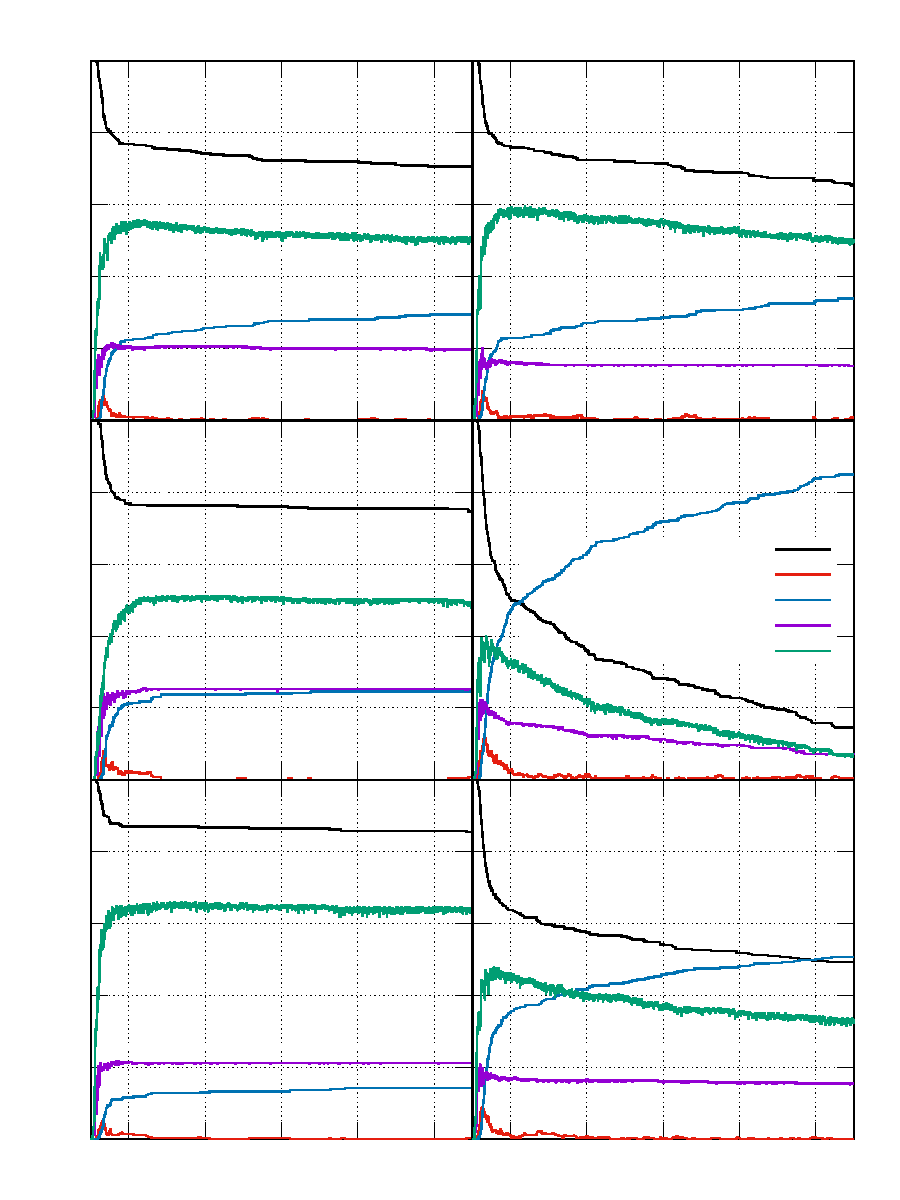
\includegraphics[width={432.00bp},height={576.00bp}]{disstot}}%
    \gplfronttext
  \end{picture}%
\endgroup
